% !TEX root = ../main.tex
\subsection*{Beryl Sea} \label{ssec::berylsea}

The Beryl Sea is a searing, tropical region, ever battered by violent winds and waters.
The region is tapered in rainforests, and it houses two of the largest nations in Yuadrem: the warring Jenkashian empire and the mysterious Gannag.
The coasts see few other countries, and seldom do ships sail in these lands.
% Apart from the two, the coasts are also inhabited by a somewhat limited variety of countries, including the ancient Edede, the resilient Voskferm, and the strange Na'ane.

% Drejeck
Westernmost of Yuadrem is the thick, dark, and moist jungle of Drejeck.
Drejeck is the birthplace of the savage naenks and the ceremonial tsaneks, and is now entirely occupied by their nation, Gannag.
Despite being born even before the Schism, the beings of Gannag are primitive and untamed, and keep their tribal ways despite regular contact with more sophisticated cultures.
The jungle is also inhabited by large and dangerous beasts that threaten the unprepared explorer, like the aggressive nadubis or the silent whowie.
% And the bulettes and the Yara-ma-yha-who.

% Fog Gorge
East to Drejeck is the Fog Gorge, a well-forested canyon island ever enveloped in fog.
While primitive, the tribes of Gannag are far from free-living, and are bound by strong shackles to their superiors.
While naenks are used to this hierarchical system, many of the more intelligent tsaneks grow tired of it over time.
A hundred and fifty years ago, a group of tsaneks went as far as to establish their own independent tribe of Na'ane in the misty island, abandoning their brethren in favor of an unrestrained lifestyle.
Freely they carry on with their ceremonies and rituals, protected from their neighbors by mist and stone.

% Qul archipelago
Further east one finds the Qul archipelago, a clump of islands that collectively served as the birth bed of the Jenkashian empire.
Jenkash is a coalition of tribes that only managed to unite after cutting down the last tree in their mountainous islands.
This led to an explosive expansion of their empire, and they swiftly conquered the neighboring lands.
Their territories now span most of the coasts of the Beryl Sea.

The archipelago itself is absolutely desolate, with barely any tree or foliage growing atop its igneous rock.
Perhaps the only bright side of this uncontrolled deforestation is the fact that it brought to light the iron and diamond veins in the eastern side of the archipelago.
These resources are heavily exploited by the qulbaba irds, and led to their signature diamond daggers.

% Dratl'fal savanna
North of the archipelago is the Dratl'fal savanna, occupied entirely by Jenkash.
The only plant that freely grows in the savanna is bafarmat, a purple moss covering its entire southeastern coast.
This plant is the primary food source of the cavernous species that live under the ichor mountains.
Its spread has allowed the hornbeetles to move into the area, a strong species of giant blue beetles that served as companions to the now ruined nation of Phrisht.

In oldentimes, the dry lands served as the birth bed for many gat city-states, of which only Dzorvepem and Jorea remain standing, now part of Jenkash.
Despite its lack of resources, the whole area was sought after by the now divided empire of Hulnar, who battled against the blooming nation of Phrisht for more than 300 years for it.
This everlasting conflict was only stopped by Jenkash, who in their thirst for conquest ended up dissolving the untiring countries.

% \begin{figure}[t]
%     \centering
%     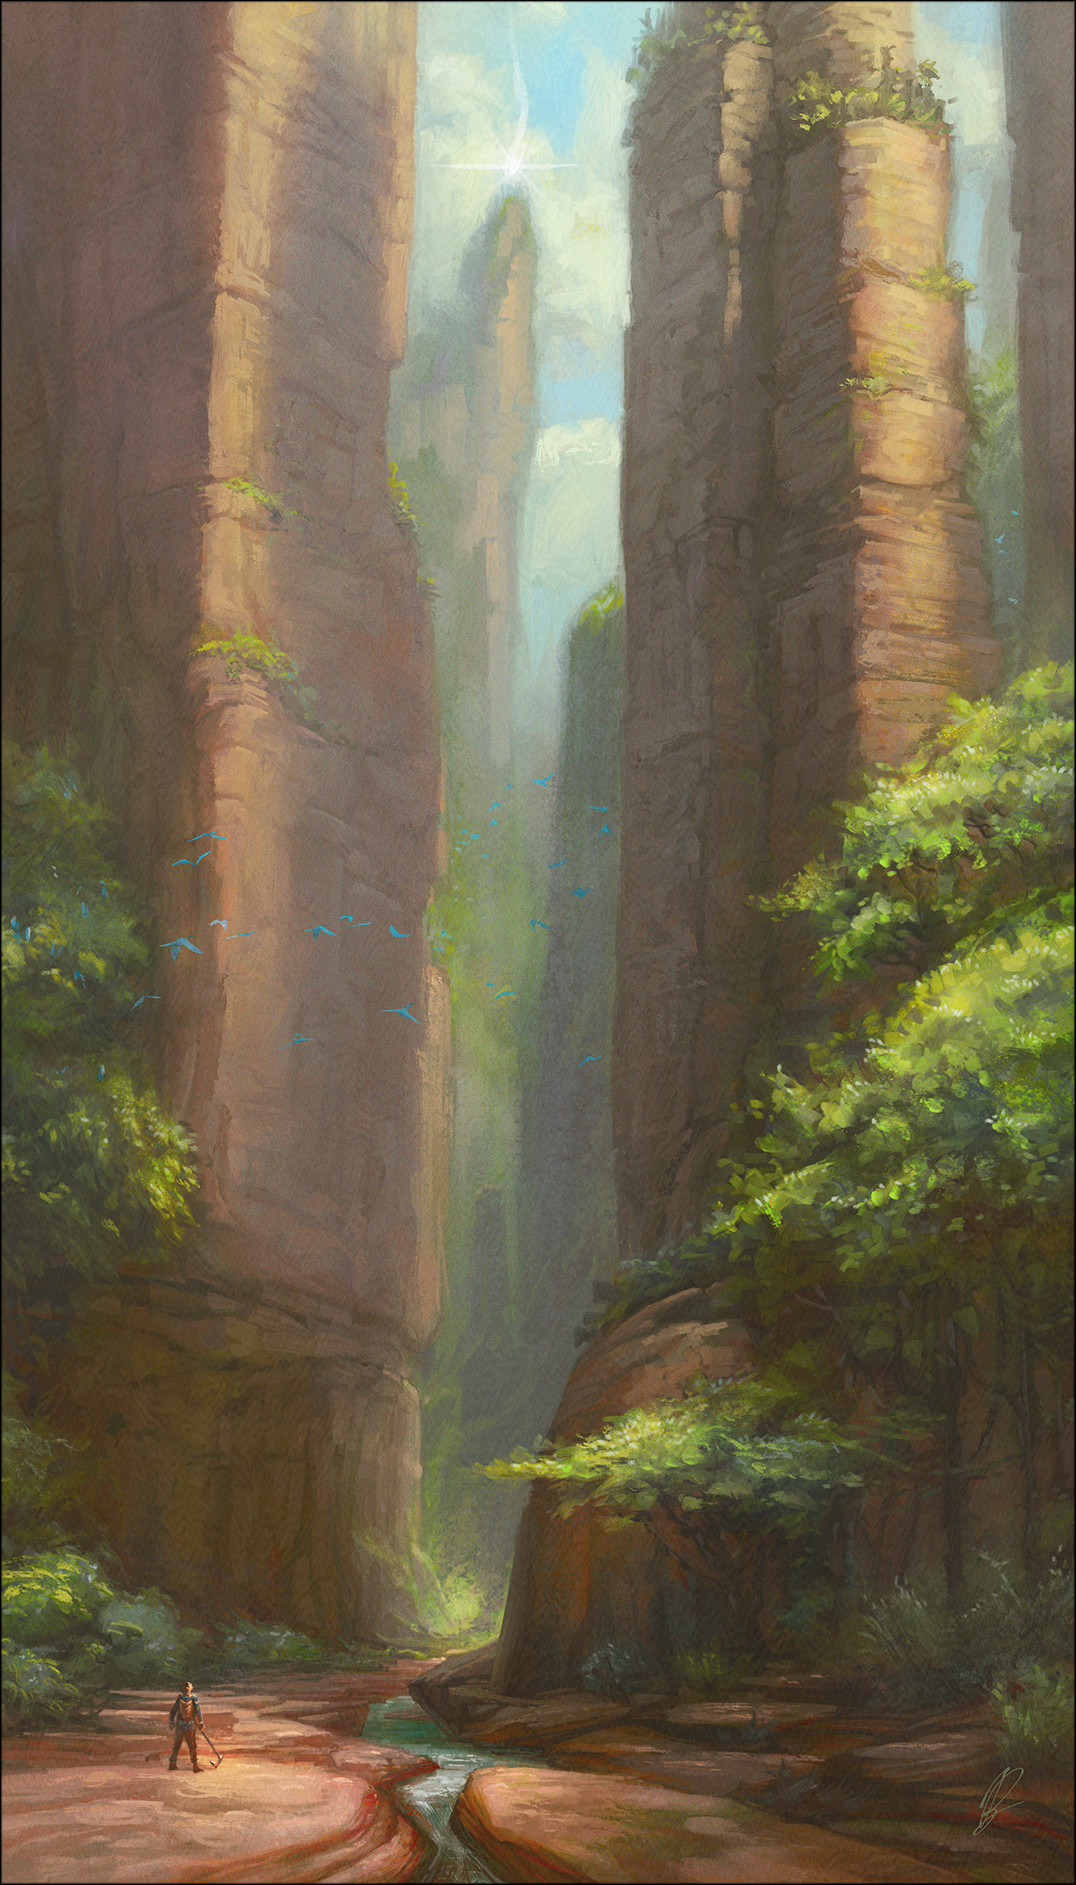
\includegraphics[width=0.46\textwidth]{01yuadrem/img/14fog_gorge.png}
%     \caption*{\centering \large{\textbf{The Fog Gorge}}}
% \end{figure}

% Ironlakes Island & Zashlath savanna
Moving to the easternmost portion of the sea one can find the Ironlakes Island and the Zashlath savanna.
The former is a large island full of forests and lakes.
It was historically a part of the peaceful marset nation of Edede, but most of it now belongs to the warring empire.
The Zashlath savanna is the area west of the desert, protected from its dry air by the moisture of the cerulean waters.
